\documentclass[10pt,twocolumn,letterpaper]{article}

\usepackage{cvpr}
\usepackage{times}
\usepackage{epsfig}
\usepackage{graphicx}
\usepackage{amsmath}
\usepackage{amssymb}

% Include other packages here, before hyperref.

% If you comment hyperref and then uncomment it, you should delete
% egpaper.aux before re-running latex.  (Or just hit 'q' on the first latex
% run, let it finish, and you should be clear).
\usepackage[breaklinks=true,bookmarks=false]{hyperref}

\cvprfinalcopy % *** Uncomment this line for the final submission

\def\cvprPaperID{****} % *** Enter the CVPR Paper ID here
\def\httilde{\mbox{\tt\raisebox{-.5ex}{\symbol{126}}}}

% Pages are numbered in submission mode, and unnumbered in camera-ready
%\ifcvprfinal\pagestyle{empty}\fi
\begin{document}

%%%%%%%%% TITLE
\title{GeReco: A deep learning approach to static and dynamic gesture recognition}

\author{Andrea Auletta\\
{\tt\small andrea.auletta@studenti.unipd.it}
\and
Marco Bernardi\\
{\tt\small marco.bernardi.11@studenti.unipd.it}
\and
Sebastiano Sanson\\
{\tt\small sebastiano.sanson@studenti.unipd.it}
}

\maketitle
%\thispagestyle{empty}

%%%%%%%%% ABSTRACT
\begin{abstract}
   This research project aims to investigate the current state of the art in gesture recognition, with an emphasis on both static and dynamic gestures. 
   It proposes an inclusive framework designed to recognize a broad spectrum of gestures, ranging from simple static gestures to complex dynamic ones. 
   The proposed framework has significant potential for applications in various domains, including human-computer interaction, robotics, and virtual reality. 
   Specific applications include human sign language recognition, gesture-based interfaces, and gesture-based game control.
\end{abstract}


%%%%%%%%% BODY TEXT
\section{Introduction}
Gesture recognition is a significant research area in computer vision and machine learning. It can be used in various applications and this is why it is an important topic to study.
The goal of this project is to study, implement and test some approaches to gesture recognition, focusing on both static and dynamic gestures: in the first one we recognize the position of 
the hand while in the second one we recognize the movement. 
We also tried to implement a real time gesture recognition system using a webcam and the developed models.
\section{Related Work}
There are many approaches to gesture recognition. Our goal was to study some of them and explore their implementation, either directly or through transfer learning, to adapt them to our problem.  
For static gesture recognition, we utilized \textit{MediaPipe Hands} \cite{zhang2020mediapipehandsondevicerealtime}, a solution developed by Google. We adapted the model by fine-tuning it to accurately classify the specific gestures required for our application.  
% PAPER -> https://iris.unimore.it/retrieve/handle/11380/1212263/282584/3DV_2020.pdf  
For dynamic gestures recognition, one of the approaches we explored in the literature was fine-tuning a \textit{Vision Transformer (ViT)}. While ViTs have shown promising results in computer vision tasks, we ultimately did not pursue this approach due to its high computational requirements and the need for large-scale training data.  
Finally, we decided to implement a custom model for dynamic gesture recognition, similar to the one proposed by Yaseen et al. \cite{electronics13163233}. This model consists of three main components: \textit{MediaPipe}, \textit{InceptionV3}, and \textit{LSTM}.  

\section{Dataset}  
The dataset is a crucial component of this project. We required two types of datasets:  

\begin{itemize}  
   \item \textbf{Dataset of static gestures}: We used a reduced version of the \textit{HaGRID dataset} \cite{Alexander_2024}.  
   The original dataset is too large for our purposes and available resources, as it contains approximately 550,000 Full-HD images (716GB) divided into 18 gesture classes.  
   Therefore, we selected a subset of about 2,000 images, distributed across 6 gesture classes.  

   \item \textbf{Dataset of dynamic gestures}: We used the \textit{Depth Camera-Based Dataset of Hand Gestures} \cite{JEERU2022108659}.  
   This dataset contains both RGB and depth video frames of various hand movements, including scroll-right/left, scroll-up/down, and zoom-in/out. Each sequence consists of 40 frames, with a total of about 700 sequences.  
   For our approach, we used only the RGB frames. To comply with the authors’ instructions, we selected 10 frames from each sequence, sampling one every 4 frames from the original 40-frames sequence.  
\end{itemize}  



\section{Method}
\subsection{Static gestures}
Mediapipe provides a good solution for hand detection and tracking. We used it to detect the hand classify the gestures.
The complex part here was to understand how to improve the accuracy of the model and we made it by using transfer learning, data augmentation and hyperparameters tuning.
\subsubsection{Data preprocessing}
For image processing it was important to choose those transformations that did not have the risk of cutting off the hands. We decided to use: \textit{rotation}, \textit{scaling}, \textit{brightness-contrast}, \textit{color conversion}, \textit{blur}, \textit{noise} and \textit{sharpening}. All these transformations were applied with random parameters.
We tried different percentages in addition to the initial dataset and the one which gave us the best results was 25\%.  
\subsubsection{Model}
Mediapipe is a framework for building pipelines to perform inference over arbitrary sensory data. This has been used to develop a model that can detect the hand and classify the gesture.
The ML pipeline of this is composed by two models working together:
\begin{itemize}
   \item \textbf{Palm detector}: operates on a full input image and locates palms via an oriented hand bounding box. The advantage of detecting the palm instead of the hand 
   is that it is a more rigid structure and it is easier to detect. The feature extraction is done via an encoder-decoder architecture. The idea is to make a recall to the 
   \textit{Feature pyramid networks} \cite{lin2017featurepyramidnetworksobject}:
   \begin{enumerate}
      \item \textit{Bottom-up pathway}: a ConvNet generates feature maps at multiple scales. The deeper layers contain more rich semantic information;
      \item \textit{Top-down pathway}: Upsample the feature maps and merge them with the corresponding feature maps through lateral connections (from the bottom-up pathway).
      This allows to recover the spatial information lost during the downsampling.
   \end{enumerate}
   \item \textbf{Hand landmark model}: operates on the cropped hand bounding box and return the landmarks. 
   The model makes a regression to estimate the coordinates of the 21 hand's landmarks. It will return also the probability of the presence of the hand and 
   the indication if the hand is left or right.
\end{itemize}
We did transfer learning on this model by training only the last layer such that it can learn to classify the gestures we needed.
For the fine-tuning of the model we tuned the \texttt{learning\_rate} and its \texttt{decay}, 
the \texttt{batch\_size}, and the \texttt{layer\_widths} in order to find a trade-off between 
efficiency and accuracy.
We \texttt{shuffled} the dataset before training in order to avoid the model to have some bias.
In order to reduce the overfitting we used the \texttt{dropout} technique to 
let the model learn different representations of the same data by setting a random fraction of 
the units of the network to 0 at each update during training time.
\subsection{Dynamic gestures}
\subsubsection{Data preprocessing}
\label{subsec:datapreprocessing}
The data preprocessing for the dynamic gestures was more complex than the one for the static gestures. As seen in the paper \cite{electronics13163233} the idea was to take 10 frames, from the video, equispaced and to crop the \textbf{region of interest (ROI) on the hands} in order to not consider useless information of the background.
After this the image should be resized to a 50x60, but InceptionV3 requires a minimum size 
of 75x75, so we decided to use those dimensions.
The idea to consider as ROI only the hands was not the best one for us, because in the dataset, the gestures were done with the whole 
arm and not only with the hands. Furthermore, not in all images mediapipe is able to recognize hands and so frames are dropped, 
but vectors of the same size are required by the \textit{LSTM}. In this way there was a big reduction of the whole dataset.
To solve these problems we tried to train the model by cropping the \textbf{ROI on pose} instead of the hands, but again the results were not good, we had a lot of frames dropped and the model was not able to classify well the gestures. \\ 
These two first techniques produce essentially an unbalanced dataset by dropping a lot of frames, furthermore we have encountered another problem, the subject in the sequence, after the cropping of the ROI and the resize of the frame, could appear stretched or squizzed, so we decided to try a third technique. \\
We tried to \textbf{not cropping the images}, but by simply removing some pixels from the margin in a way to have all the body of the person in the image and less background.
\subsubsection{Model}
The pipeline is similar to the one explained by Yaseen et al \cite{electronics13163233}, it is composed by three main parts:
\begin{enumerate}
   \item \textbf{MediaPipe}: MediaPipe is used to detect and then crop the ROI from each frame of the video.
   As said in the previous section \ref{subsec:datapreprocessing} we have tried to train the model considering 
   different regions of interest. We tried to crop the hand and the body of the person in the video. 
   \item \textbf{InceptionV3}: we used the InceptionV3 model \cite{szegedy2015rethinkinginceptionarchitecturecomputer} 
   to extract features from the cropped regions of interest.
   The idea of Inception is to have filters with different sizes in the same layer and then concatenate 
   the results. What is trying to solve InceptionV3 with respect to the previous versions are:
   \begin{itemize}
      \item \textit{Reducing the representational bottleneck}: neural networks perform better when convolutions
      didn't alter the dimension of the input drastically, there could be a loss of information;
      \item \textit{Using smart factorization network}
   \end{itemize}  
   These problems are solved by \textit{factorizing filters} (e.g. 5x5 in two of 3x3) and by \textit{expanding 
   the banks of filter in a wider way} instead of having deeper networks. 
   Deeper models means higher reduction and hence loss of information.
   \item \textbf{LSTM}: we used a LSTM layer to classify the gestures. 
   The LSTM is a type of RNN, this means that can take in input a sequence of data. This is useful in our case
   because we are trying to classify a sequence of frames. In the simple RNN there is an internal memory 
   that allows to remember the previous results and the computation of the current input depends on 
   the previous one. The problem with the simple RNN is that it has a problem with the \textit{vanishing gradient}.
   LSTM solves this problem by introducing different components which allows to keep the information 
   for a longer time (forget gate, input gate, output gate).
\end{enumerate}
The only model we trained on here is the LSTM model. The main problem we found during the training 
was the overfitting. We tried to solve this problem by using:
\begin{itemize}
   \item \textit{Dropout}: it reduces the overfitting because the network is forced to learn different representations of the same data;
   \item \textit{L2 regularization}: it works by adding a penalty to the loss function;
   \item \textit{early stopping}: it works by stopping the training when the validation loss 
   has no improvement for a certain number of epochs. We set the number of \textit{epochs} to 
   300 and for our purposes there were too many since it overfitted after fewer epochs;
   \item \textit{Batch normalization}: it works by normalizing the input of the layer in order to have normalized data with zero mean and unit variance.
\end{itemize}
We also found here a trade-off between efficiency and accuracy by tuninig 
the \textit{batch size} and the \textit{learning rate}.

\section{Experiments}
\subsection{Static gestures}
In the following table \ref{tab:staticGestures} we can see the results of the model 
trained on the static gestures dataset. 
The tests are splitted based on the percentage of the augmented dataset with reference to number of the examples.
\begin{table}[h]
   \begin{center}
   \begin{tabular}{|c|c|c|c|c|}
   \hline
   \textbf{Aug. \%} & \textbf{Val\_loss} & \textbf{Val\_Acc.} & \textbf{Test\_loss} & \textbf{Test\_Acc.}\\
   \hline\hline
   20 & 0.13 & 0.90 & 0.17 & 0.87 \\
   \textbf{25} & 0.16 & 0.89 & \textbf{0.13} & \textbf{0.90} \\
   30 & 0.19 & 0.86 & 0.19 & 0.87 \\
   35 & 0.16 & 0.88 & 0.19 & 0.88 \\
   40 & 0.18 & 0.86 & 0.17 & 0.87 \\
   100 & 0.22 & 0.84 & 0.19 & 0.87 \\ 
   \hline
   \end{tabular}
   \end{center}
   \caption{Results of the model trained on the static gestures dataset.}
   \label{tab:staticGestures}
\end{table} \\
We can say that the best results for the test accuracy are obtained with the 25\% of the 
augmented dataset, intrducing enough variability in the dataset in order to 
improve the robustness of the model, but not too much to make data too different from the original one.
At lower percentages the model could not have seen enough variations in the data to generalize well, and at 
higher percentages the model could have seen too many variations making the learning less effective.
\subsection{Dynamic Gestures}
The initial experiment aimed to replicate the behavior of the model proposed by Yaseen et al. \cite{electronics13163233}, using the same dataset split and hyperparameters.  
The results showed that the performance metrics were similar to those obtained by the authors. 
However, despite achieving high test accuracy, the model failed to correctly classify gestures 
in a live-stream test environment.  

Our initial hypothesis was that cropping images around the hands might not be the optimal approach. By focusing solely on the hands, the model lost crucial contextual information related to the gesture, particularly the position of the arms and the movement of the body.
To address this issue, we leveraged MediaPipe pose detection to refine the cropping strategy, using keypoints as regions of interest (ROI). However, this modification did not lead to significant improvements in classification performance.  

These findings suggest that the issue was not related to the cropping strategy.  

\subsubsection{The Dataset Problem}
Further research highlighted that the issue stemmed from the dataset. The dataset was not properly split between training and testing.  
Due to the nature of the examples, some samples were very similar to each other, leading the model to potentially classify gestures based on background and the color of the subject’s clothing rather than their actual motion.  
This resulted in high metric values but poor generalization.  
Ad that the dataset was not well splitted, we decided to manually split (instead of using a random split) the dataset in order to have clearly different examples between train and test.

\subsubsection{Results}
Initially, we were able to replicate the results obtained by Yaseen et al. \cite{electronics13163233}
as shown in Table \ref{tab:dynamicGesturesBad}, but only when using an incorrect dataset split.  
\begin{table}[h]
   \begin{center}
   \begin{tabular}{|c|c|c|c|c|}
   \hline
   \textbf{Cropping} & \textbf{Val\_loss} & \textbf{Val\_Acc.} & \textbf{Test\_loss} & \textbf{Test\_Acc.}\\
   \hline\hline
   Hands & 0.32 & 0.91 & 0.33 & 0.92 \\
   Pose & 2.15 & 0.89 & 2.18 & 0.90 \\
   \hline
   \end{tabular}
   \end{center}
   \caption{Best results of the model trained on the bad splitted dynamic gestures dataset.}
   \label{tab:dynamicGesturesBad}
\end{table} \\
This suggests that the original high accuracy was likely influenced by data leakage, where similar examples appeared in both the training and test sets. 

After manually restructuring the dataset to ensure a clear separation between training and test samples, we observed a significant drop in accuracy. 
(see Table \ref{tab:dynamicGesturesWell}).
However, this decline indicated a more realistic performance evaluation, 
revealing the model's actual inability to generalize unseen gestures.  
These findings emphasize the importance of a well-structured dataset split when evaluating deep 
learning models, particularly in gesture recognition tasks.
% DATI TABELLA DA SISTEMARE %%%%%%%%%%%%%%%%%%%%
\begin{table}[h]
   \begin{center}
   \begin{tabular}{|c|c|c|c|c|}
   \hline
   \textbf{Cropping} & \textbf{Val\_loss} & \textbf{Val\_Acc.} & \textbf{Test\_loss} & \textbf{Test\_Acc.}\\
   \hline\hline
   Hands & 2.05 & 0.63 & 1.69 & 0.76 \\
   No crop & 0.69 & 0.91 & 1.95 & 0.53 \\
   \hline
   \end{tabular}
   \end{center}
   \caption{Best results of the model trained on the well splitted dynamic gestures dataset.}
   \label{tab:dynamicGesturesWell}
\end{table}
A thing that we can say about the dataset based on the crop of the hands is that it was to small for the 
fact that mediapipe was not able to recognize the hands in all the frames of the videos, and the model 
could not have seen enough variations in the data to generalize well. \\
\begin{figure}[h]
   \centering
   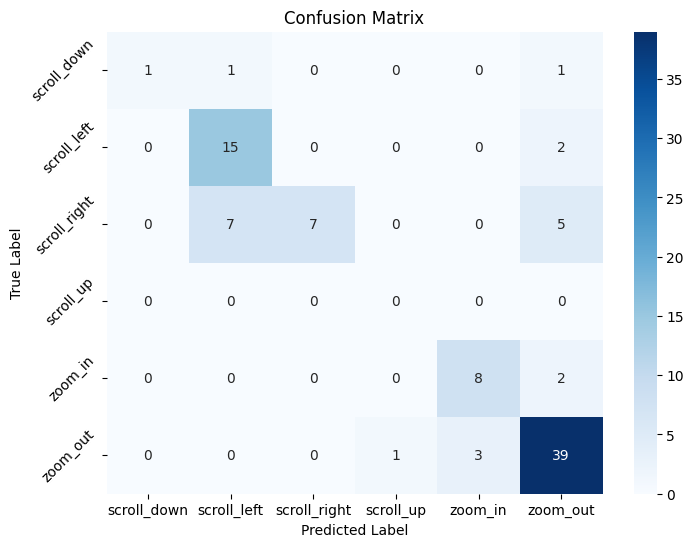
\includegraphics[width=1\linewidth]{images/rightDatasetHandsCrop.png}
   \caption{Confusion matrix of the model trained with the hands cropped dataset.}
   \label{fig:handCropConfusionMatrix}
\end{figure}
Also in the confusion matrix presented \ref{fig:handCropConfusionMatrix} we can see that a lot of immages 
were lost during the preprocessing. We can see that the model is able to well classify only three classes out 
of six.

For the images without crop we can see that the accuracy is quite low and the model is not 
able again to classify well all the types of gestures.
\begin{figure}[h]
   \centering
   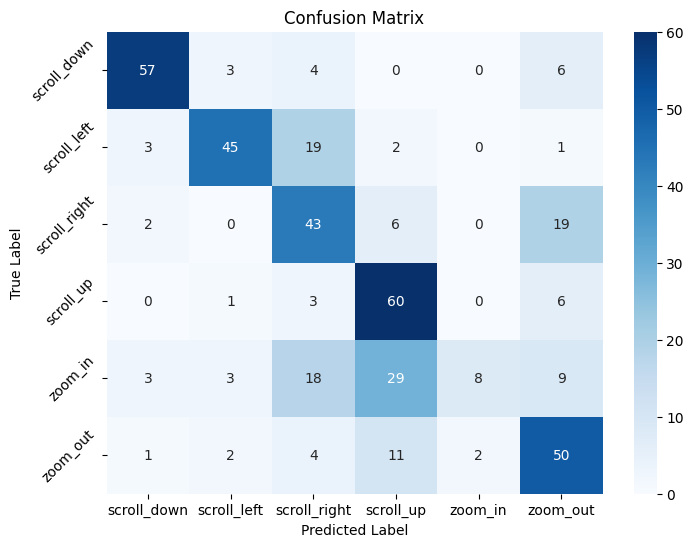
\includegraphics[width=1\linewidth]{images/matrix_confusion2.png}
   \caption{Confusion matrix of the model trained with the no crop dataset.}
   \label{fig:noCropConfusionMatrix}
\end{figure} \\
In the confusion matrix presented \ref{fig:noCropConfusionMatrix} we can clearly see 
that examples are not dropped and some gestures are classified better than others like the zoom-out 
or the scroll-left. In a real time recognition system this second model worked better than the 
first one, but the accuracy was still too low to be used in a real application.

\section{Conclusion and future works}
In this project we focused more on the modification of the dataset to recover frames lost 
during the preprocessing instead of finding a way to choose other frames, so this is 
a possible work to do to improve the model.
We can say that with more resources we could get better results in less time, 
specially for the dynamic gestures:
\begin{itemize}
   \item \textbf{Camera} for the real time recognition;
   \item \textbf{GPU} for the training of the models;
   \item \textbf{Memory} to store more data and process all the frames of the videos.
\end{itemize}
The model for the static gesture recognition worked well and thanks to the transfer learning 
we were able to get good results in a short time. The model for the dynamic gesture recognition
was more complex, it has been necessary a deep study on the dataset and the preprocessing and a lot of time 
and run trying to get the best possible results.

{\small
\bibliographystyle{ieee_fullname}
\bibliography{egbib}
}

\end{document}
